\documentclass[10pt,a4paper,oneside]{article}
\usepackage[utf8]{inputenc}
\usepackage[T1]{fontenc}
\usepackage{amsmath}
\usepackage{amsfonts}
\usepackage{amssymb}
\usepackage{enumerate}
\usepackage{graphicx}
\usepackage{tikz}

\date{June 10, 2019}
\author{Baboo J. Cui}
\title{Linear Quadratic Regulator(LQR) for Discrete-Time System}
\begin{document}
\maketitle
\tableofcontents

\newpage

LQR is related to optimal control problem, many problems can be formulated into it. It's one of the fundamental ways to achieve optimal control.

\section{Problem Formulation and Direct Solution}
Given a discrete LTI system:
\[
x[k+1] = Ax[k] + Bu[k], x[0] = x_0
\]
given a time horizon $k \in \{0, 1, \dots, N\}$, where $N$ may be infinity, find the optimal input sequence $U = \{u[0], u[1], \dots, u[N-1]\}$ that minimize the \textbf{cost function}:
\[
J(U) = \underbrace{\sum_{k=0}^{N-1}\left(x^T[k] Qx[k] +u^T[k] Ru[k]\right)}_{\text{running cost}} + \underbrace{x^T[N]Q_f x[N]}_{\text{terminal cost}}
\]

\begin{itemize}
	\item \textbf{state weight matrix}: $Q = Q^T \succeq 0$
	\item \textbf{control weight matrix}: $R = R^T \succ 0$, indicate that there is no free control input
	\item \textbf{final state weight matrix}: $Q_f = Q_f^T \succeq 0$
	\item \textbf{running cost}: for time horizon from $1$ to $N-1$
	\item \textbf{terminal cost}: for time at $N$
	\item \textbf{infinite case}: $N$ is infinity, in this case, $Q_f = 0$
\end{itemize}
Here is the direct solution:
\begin{itemize}
	\item suppose value function at time $t+1$ is \textbf{quadratic}: $V_{t+1}(x)=x^TP_{t+1}x$, then value function at time $t$ is also \textbf{quadratic}:
	\[
	V_t(x)=x^T P_t x, \forall x\in \mathbb{R}^n
	\]
	\item $P_t$ can be obtained from $P_{t+1}$ according to the \textbf{Riccati recursion}:
	\[
	P_t=Q+A^TP_{t+1}A - A^TP_{t+1}B(R+B^TP_{t+1}B)^{-1}B^TP_{t+1}A
	\]
	\item minimum value of $J$ is $J^* = x_0^T P_0 x_0$
	\item optimal control at time $t$ for the given state $x[t]=x$ is:
	\[
	u^*[t] = -\underbrace{(R+B^T P_{t+1} B)^{-1}B^T P_{t+1} A }_{\text{Kalman gain } K} x= - K_tx
	\]
	which is a \textbf{linear state feedback} control
\end{itemize}
Note that it can be \textbf{generalized} into time-varying cases by setting $A, B, Q, R$ into is time varying counterparts $A(t), B(t), Q(t), R(t)$. Here $A(t)$ should be used instead of $A(t+1)$.


\section{Examples of Implementations}
Many problem can be formulated into LQR form, and here are some examples, though they look differently in format.

\subsection{Energy Efficient Stabilization}
Starting from $x[0] = x_0$, find control sequence $U$ that minimize
\[
J(U) = \alpha \sum_{k=0}^{n-1} || u[k] ||^2 + \beta \sum_{k=0}^{N} || x[k] ||^2
\]
to make it into LQR form, choose:
\begin{itemize}
	\item $Q = \beta I$
	\item $R = \alpha I$
	\item $Q_f = \beta I$
\end{itemize}
Note that:
\begin{itemize}
	\item cost function try to make state trajectory stay close to zero and use the least control energy simultaneously
	\item $\alpha$ and $\beta$ determine the emphasis, can be adjusted
\end{itemize}
Sometimes state cannot be obtained directly, and system \textbf{output} $y$ can be used for evaluating running cost. Suppose output equation($Du$ part can be eliminate) is
\[
y = Cx
\]
in this case choose 
\[
Q = \beta C^T C
\]
 Here is the proof:
\begin{align*}
\beta \sum_{k=0}^{N} || y[k] ||^2 &=  \sum_{k=0}^{N} y^T [k] \beta I y[k]\\
&= \sum_{k=0}^{N} (Cx[k])^T \beta I Cx[k]\\
&= \sum_{k=0}^{N} x^T[k] C^T \beta I Cx[k] = \sum_{k=0}^{N} x^T[k] (\beta C^T C)x[k]
\end{align*}
this is a useful conclusion for reformation.

\subsection{Minimum Energy Steering}
Starting from $x[0] = x_0$, find control sequence $U$ to use least energy to steer the final state to $x[N] = 0$ without lost generosity, the cost is:
\[
J(U) = \sum_{k=0}^{N-1} ||u[k]||^2
\]
to make it into LQR form, choose:
\begin{itemize}
	\item $Q = 0$
	\item $R =  I$
	\item $Q_f = \infty I$
\end{itemize}
By setting $Q_f \rightarrow \infty I$, there is a big penalty if $X[N]$ is far from $0$. This won't lead to a analytic solution, but the \textbf{approximation} is good enough. 

\subsection{LQR for Tracking(VIP TOPIC)}
Find efficient sequence $U$ for the state to track a given\textbf{ reference trajectory} $x_k^*$(may be time-varying):
\[
J(U) = \alpha \sum_{k=0}^{N-1} ||u[k]||^2 + \beta \sum_{k=0}^{N} ||x[k] - x_k^*||^2
\]
note that $||x[k] - x_k^*||^2$ is not homogeneous quadratic, it should be formulate. It can be expanded(refer math proof in last part) as:
\begin{align*}
||x[k] - x_k^*||^2 &= x^T[k] x[k] -2x^T[k]x_k^* + (x_k^*)^T x_k^*\\
&=\begin{bmatrix}
x^T[k] & 1
\end{bmatrix}
\begin{bmatrix}
I & x_k^*\\
(x_k^*)^T &  (x_k^*)^T x_k^*
\end{bmatrix}
\begin{bmatrix}
x[k]\\ 1
\end{bmatrix} \quad \text{dimension augmentation}
\end{align*}
construct new state variable $\tilde{x}[k] = [x[k]\quad 1]^T$, new system dynamic will be:
\[
\tilde{x}[k+1] = \begin{bmatrix}
A & 0 \\ 0& 1
\end{bmatrix} \tilde{x}[k] + \begin{bmatrix}
B \\ 0
\end{bmatrix} u[k]
\]
and the origin cost can be reformed as:
\[
J(U) = \alpha \sum_{k=0}^{N-1} ||u[k]||^2 + \beta \sum_{k=0}^{N} \tilde{x}^T[k] \tilde{Q}_k \tilde{x}[k] 
\]
where
\[
\tilde{Q}_k = \begin{bmatrix}
I & x_k^*\\
(x_k^*)^T &  (x_k^*)^T x_k^*
\end{bmatrix}
\]
clearly, the system is LTI and the cost function is LTV.

\subsection{LQR for System with Perturbation}
Suppose system is:
\[
x[k+1] = Ax[k] + Bu[k] + w[k]
\]
To achieve LQR formulation, new state vector is constructed as:
\[
\tilde{x}[k] = [x^T[k] \quad z[k]] \quad \text{dimension augmentation}
\]
recall that $x \in \mathbb{R}^n$, and $z[k] \in \mathbb{R}$, set $z[k] = z[k+1] =1$, new system dynamic will be:
\[
\tilde{x}[k+1] = \begin{bmatrix}
A & w[k] \\ 0& 1
\end{bmatrix} \tilde{x}[k] + \begin{bmatrix}
B \\ 0
\end{bmatrix} u[k]
\]
and system initial condition is $\tilde{x}[0] = [x[0] \quad 1]$. $R$ will be the original one and $\tilde{Q}$ is:
\[
\tilde{Q}_k = \begin{bmatrix}
Q & 0\\
0 & 0
\end{bmatrix}
\]
clearly, the system is LTV and the cost function is LTI. In this case, $u$ is not changed, $x$ is augmented.

\section{Direct Approach to Solve LQR}
LQR can directly be formulated as a least square problem, although this is not recommended, however it offers us very import conclusions.

\subsection{Reconstruct the Problem}
The system dynamics  can be augmented to a big equation:
$$
\underbrace{\left[\begin{array}{c}{x[1]} \\ {x[2]} \\ {\vdots} \\{x[N]}\end{array}\right]}_{\tilde{X}}
=
\underbrace{\left[\begin{array}{cccc}
	{B} & {0} & {\cdots} & {\cdots} \\ 
	{A B} & {B} & {0} & {\cdots}  \\ 
	{\vdots} & {\vdots} & {\ddots} & {\cdots} \\ 
	{A^{N-1} B} & {A^{N-2} B} & {\cdots} & {B}\\
	\end{array}\right]}_{\tilde{G}}
\underbrace{\left[\begin{array}{c}{u[0]} \\ {u[1]} \\ {\vdots} \\ {u[N-1]}\end{array}\right]}_{\tilde{U}}+
\underbrace{\left[\begin{array}{c}{A} \\ {A^{2}} \\ {\vdots} \\ {A^{N}}\end{array}\right]}_{\tilde{H}} x_{0}
$$
Recall that $\title{G}\tilde{U}$ is the zero-state response and $\tilde{H}x_0$ is the zero-input response and the cost function can be rewrite as:
\[
J(U) = 
\tilde{X}^T\underbrace{\left[\begin{array}{cccc}
	{Q} & {} & {} & {} \\ 
	{} & {Q} & {} & {} \\ 
	{} & {} & {\ddots} & {} \\ 
	{} & {} & {} & {Q_f}\end{array}\right]}_{\tilde{Q}} \tilde{X}+
\tilde{U}^T\underbrace{\left[\begin{array}{cccc}
	{R} & {} & {} & {} \\ 
	{} & {R} & {} & {} \\ 
	{} & {} & {\ddots} & {} \\
	 {} & {} & {} & {R}\end{array}\right]}_{\tilde{R}}\tilde{U}
\]
And the problem can be written in a compact form as:
\begin{align*}
\min \quad &\tilde{X}^T \tilde{Q} \tilde{X} + \tilde{U}^T \tilde{R} \tilde{U}\\
\text{s.t.} \quad &\tilde{X} = \tilde{G} \tilde{U} + \tilde{H}x_0
\end{align*}

\subsection{Directly Solve the Reconstructed Problem}
There are two ways to solve this problem:
\begin{itemize}
	\item Lagrange multiplier approach
	\item plug the equality constraint into cost function to form an unconstrained optimization problem(here we use this way)
\end{itemize}
By substituting equality constraints into the cost function:
\begin{align*}
J(\tilde{U}) &= (\tilde{G} \tilde{U} + \tilde{H}x_0)^T \tilde{Q} (\tilde{G} \tilde{U} + \tilde{H}x_0) + \tilde{U}^T \tilde{R} \tilde{U}\\
&= \tilde{U}^T \tilde{G}^T \tilde{Q} \tilde{G} \tilde{U} + \tilde{U}^T \tilde{G}^T \tilde{Q} \tilde{H} x_0 + x_0 \tilde{H}^T  \tilde{Q} \tilde{G} \tilde{U} + x_0 \tilde{H}^T  \tilde{Q} \tilde{H} x_0 + \tilde{U}^T \tilde{R} \tilde{U}\\
&= \tilde{U}^T (\tilde{G}^T \tilde{Q} \tilde{G} +\tilde{R})\tilde{U} + 2 \tilde{U}^T \tilde{G}^T \tilde{Q} \tilde{H} x_0 + x_0 \tilde{H}^T  \tilde{Q} \tilde{H} x_0
\end{align*}

To find the $U$ that minimize $J$, take the first order derivative:
\[
\frac{d J(\tilde{U})}{d \tilde{U}} = 2 (\tilde{G}^T \tilde{Q} \tilde{G} +\tilde{R})\tilde{U} + 2 \tilde{G}^T \tilde{Q} \tilde{H} x_0
\]
By setting it to $0$ can we find the optimal $\tilde{U}$ since it has only one solution:
\[
\tilde{U}^* = -(\tilde{G}^T \tilde{Q} \tilde{G} +\tilde{R})^{-1} \tilde{G}^T \tilde{Q} \tilde{H} x_0
\]

\subsection{Limitations of Direct Approach}
\begin{itemize}
	\item matrix inversion is needed to find optimal control
	\item matrices dimension increases with time horizon $N$
	\item impractical for large $N$, impossible for infinite time horizon case 
	\item sensitivity of solutions to numerical errors
\end{itemize}

\subsection{Observations from Direct Approach}
\begin{itemize}
	\item easier to solve for shorter time horizon $N$
	\item $(N+1)$-horizon solution related to $N$-horizon solution, iterative solution could be feasible
	\item optimal control sequence has \textbf{linear feedback form}
\end{itemize}

\section{Dynamic Programming}

\subsection{Dynamic programming approach}
\begin{itemize}
	\item reuse results for smaller $N$ to solve for large $N$ case
	\item each iteration only need to deal with a problem of fixed size
\end{itemize}

\subsection{Motivating Example}
Start from point $A$, try to reach point $B$, each step only move right and cost labeled on each edge. How to find the least costly path from A to B?
\begin{center}
	\begin{tikz}
		\draw(0,0) grid [rotate=45](3,3)
		node at (-2.4,2.1) {A} 
		node at (-1.6,1.8) {7}
		node at (-1.6,2.4){5}
		node at (-0.9,2.5){8}
		node at (-0.9,3.1){6}
		node at (-0.9,1.7){7}
		node at (-0.9,1.1){9}
		node at (-0.2,1 ){10}
		node at (-0.2,0.4){6}
		node at (-0.2,2.4){10}
		node at (-0.2,1.8){8}
		node at (-0.2,3.2){6}
		node at (-0.2,3.8){10}
		node at (0.5,0.3){7}
		node at (0.6,1.1){12}
		node at (0.5,1.7){5}
		node at (0.5,2.5){9}
		node at (0.5,3.1){5}
		node at (0.5,3.9){7}
		node at (1.2,1){9}
		node at (1.2,1.8){7}
		node at (1.2,2.4){6}
		node at (1.2,3.2){8}
		node at (1.9,1.6){11}
		node at (1.9,2.6){10}
		node at (2.4,2.1){B};
	\end{tikz}
\end{center}
This can be formulated as an optimal control problem, each node may be assigned by a coordinate, specifically:
\[
A=(0, 0) \quad B=(3, 3)
\]
state $x[k]$ with boundary condition: $x[0]=A$, and $x[6]=B$. Control input is $u[k]=\pm1$, and system dynamics is
\[
x[k+1]=\left\{\begin{array}{ll}{x[k]+(0,1)} & {u[k]=1} \\
{x[k]+(1,0)} & {u[k]=-1}\end{array}\right.
\]
Cost to be minimized:
\[
\sum_{k=0}^{5} w(x[k], u[k])
\]
where $w$ is the edge weight(or edge cost).

\subsection{Direct Solution}
Enumerate all possible legal from $A$ to $B$ and compare their costs to find the least cost.
\begin{itemize}
	\item for $\ell$-by-$\ell$ grid, the total number of legal paths is
	$$
	\frac{(2 \ell) !}{(\ell !)^{2}}
	$$
	\item grows extremely fast as problem size $\ell$ increases, beyond exponential bound
	\item solution impractical for large $\ell$
	\item solution \textbf{impossible} when input is \textbf{infinite}
\end{itemize}

\subsection{Value Function(VIP)}
At any point(state in a more general case) $z$, the \textbf{value function}(optimal cost-to-go) $V(z)$ is the least possible cost to reach terminal($B$ in motivating example) from $z$. Note that:
\begin{itemize}
	\item $V(z)$ can be obtained by solve \textbf{shorter} time horizon problems
	\item original problem can be formulated as to find $V(A)$
\end{itemize}
So optimal control problem can be transformed into value function problem.

\subsection{Principle of Optimality(VIP)}
If a least-cost path from $A$ to $B$ is
\[
x^*_0=A\rightarrow x^*_1\rightarrow x^*_2\rightarrow\dots\rightarrow x^*_6=B,
\]
then any truncation of it at the end:
\[
x^*_t\rightarrow x^*_{t+1}\rightarrow \dots \rightarrow x^*_6=B
\]
is also a least-cost path from $x^*_t$ to B. As a result:
\[
\begin{aligned} 
V(z) &=\min \left\{w_{u}+V\left(z_{u}^{\prime}\right), w_{d}+V\left(z_{d}^{\prime}\right)\right\} \\
 &=\min _{u \in \pm 1}\left[w(z, u)+V\left(z^{\prime}\right)\right] \end{aligned}
\]
\begin{center}
	\begin{tikz}
		\draw(0,0) grid [rotate=45](1,1)
		node at (-1,0.7) {$z$} 
		node at (0,1.7){$z'_u$}
		node at (0,-0.3){$z'_d$}
		node at (-0.5,1.3){$w_u$}
		node at (-0.5,0.1){$w_d$};
	\end{tikz}
\end{center}
\begin{itemize}
	\item $V(z)$: minimum cost-to-go from current position
	\item $w(z,u)$: running cost of current step
	\item $V(z^{\prime})$: cost-to-go from next state position
\end{itemize}
And the motivating problem can be solved by \textbf{iteration} from final to initial point.

\subsection{Advantages of Dynamic Programming}
\begin{itemize}
	\item only need to compute $\ell^2$ value functions(P-problem)
	\item no need to enumerate $\frac{(2\ell)!}{(\ell!)^2}$ paths(avoid NP problem)
	\item solve an optimization problem of fixed size in each iteration
	\item even if starting from a different initial position (e.g. due to perturbation), there is no need for re-computation(a family of problems can be solved)
\end{itemize}

\section{Solve LQR Problem by Dynamic Programming}
Recall LQR problem formulation: a discrete-time LTI system
\[
x[k+1]=Ax[k]+Bu[k],x[0]=x_0
\]
Given a time horizon $k\in\{0,1,...,N\}$, find the optimal input sequence $U=\{u[0],...,u[N-1]\}$ that minimizes the cost function
\[
J(U)=\sum_{k=0}^{N-1}(x^T[k] Q x[k]+u^T[k] R u[k])+x^T[N] Q_f x[N]
\]

\subsection{Value Function of LQR Problem}
The value function at any time $t\in\{0,1,...,N\}$ and state $x\in\mathbb{R}^n$ is
\[
V_t(x)=\min_{u[t],...,u[N-1]}\sum_{k=t}^{N-1}(x^T[k] Q x[k]+u^T[k] R u[k])+x^T[N] Q_f x[N]
\]
with the initial condition $x[t]=x$, namely, \textbf{cost-to-go} $V_t(x)$ is optimal cost of the LQR problem over the time horizon $\{t,t+1,...,N\}$, starting from $x[t]=x$(arbitrary). Note that:
\[
V_0(x) = J(U)
\]

\subsection{Solution of LQR Problem via Value Functions}
Preview of results:
\begin{itemize}
	\item the value function at the final time is quadratic: $V_N(x)=x^T Q_f x$
	\item the value function at any time $t$ is also \textbf{quadratic}: $V_t(x)=x^T P_t x$ for \textbf{some} $P_t \succeq 0$,(the proof is in extra part)
	\item $P_t$ can be obtained from $P_{t+1}$ \textbf{recursively}
\end{itemize}
\textbf{Solution algorithm(VIP)}:
\begin{enumerate}
	\item start from $P_N = Q_f$ at time $t=N$
	\item for $t = \{N-1, N-2, \dots, 0\}$, compute $P_t$ from $P_{t+1}$ by the above recursion
	\item recover optimal control sequence from value functions
\end{enumerate}

\subsection{Recursion of Value Functions(VIP)}
\textbf{Hamilton-Jacobi-Bellman(HJB) equation}:
\[
\begin{aligned}
V_t(x) &= \min_{u[t]=v}[x^TQx+v^TRv+V_{t+1}(Ax+Bv)]\\
&= x^TQx+\min_{u[t]=v}[v^TRv+V_{t+1}(Ax+Bv)]
\end{aligned}
\]
Optimality principle: for optimal case, cost-to-go from next state $x[t+1]$, i.e. $V_{t+1}(x[t+1])$, should also be optimal. \\
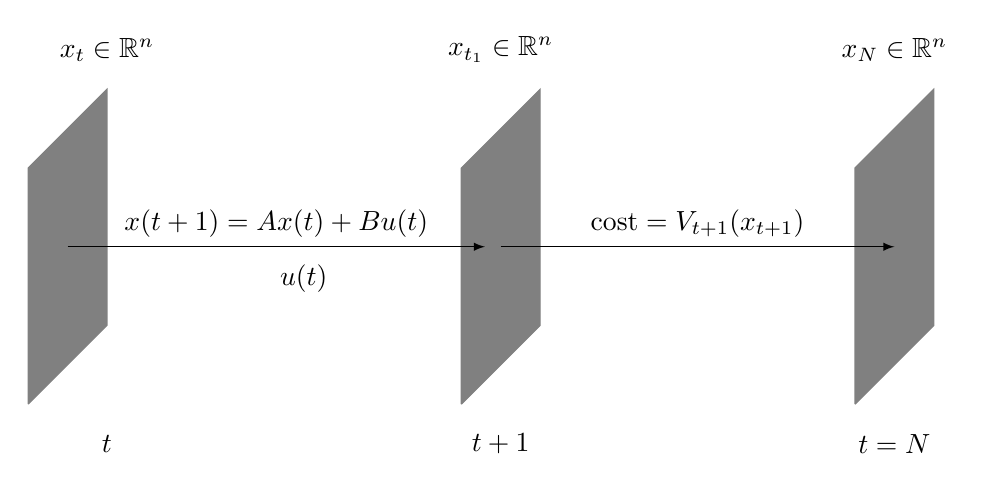
\begin{tikzpicture}[auto,>=latex]
\filldraw[gray] (-0.5,0)--(-0.5,3)--(0.5,4)--(0.5,1)--(-0.5,0);
\filldraw[gray] (5,0)--(5,3)--(6,4)--(6,1)--(5,0);
\filldraw[gray] (10,0)--(10,3)--(11,4)--(11,1)--(10,0);
\draw node at (0.5,-0.5) {$t$};
\draw node at (5.5,-0.5) {$t+1$};
\draw node at (10.5,-0.5) {$t=N$};
\draw node at (0.5,4.5) {$x_t\in\mathbb{R}^n$};
\draw node at (5.5,4.5) {$x_{t_1}\in\mathbb{R}^n$};
\draw node at (10.5,4.5) {$x_N\in\mathbb{R}^n$};
\draw node at (3, 1.6) {$u(t)$};
\draw[->](0,2)-- node {$x(t+1)=Ax(t)+Bu(t)$}(5.3,2);
\draw[->](5.5,2)-- node {$\text{cost}=V_{t+1}(x_{t+1})$}(10.5,2);
\end{tikzpicture}
And here is the process:
\begin{enumerate}
	\item \textbf{$t=N$ case}: value function is quadratic and can be directly found as:
	\[
	V_N(x)=x^T P_N x = x^T Q_f x,\forall x\in \mathbb{R}^n,\text{where }P_N=Q_f
	\]
	\item \textbf{$t=N-1$ case}:
	\[
	\begin{aligned}
	V_{N-1}(x) &= x^T Q x + \min_{v}[v^T R v+V_N(Ax+Bv)]\\
	&= x^T Q x + \min_{v}[v^T R v+(Ax+Bv)^T P_N (Ax+Bv)]
	\end{aligned}
	\]
\end{enumerate}
First to prove that optimal controller has linear state feed back form:
\begin{align*}
V_{N-1}(x) &= x^T Q x + \min_{v}[v^T R v+V_N(Ax+Bv)]\\
&= x^T Q x + \min_{v}[v^T R v+(Ax+Bv)^T P_N (Ax+Bv)] \quad \text{quadratic expansion}\\
&= x^T Q x + \min_{v}[v^T R v+ x^TA^TP_NAx + 2v^TB^TP_NAx + v^TB^TP_NBv] \quad \text{move out term}\\
&=  x^T Q x + x^TA^TP_NAx + \min_{v}[v^T R v  + 2v^TB^TP_NAx + v^TB^TP_NBv] \quad \text{combine like terms}\\
&= x^T(Q+A^TP_NA)x + \min_{v}[2v^TB^TP_NAx + v^T (R + B^TP_NB)v]
\end{align*}
o find the optimal $u*=v$, take derivative of the terms in $\min$ function to $v$ and set to $0$:
\begin{align*}
\frac{\partial}{\partial v} \left(2v^TB^TP_NAx + v^T (R + B^TP_NB)v\right) &= 0\\
2 B^TP_NAx + 2 (R + B^TP_NB)v^*  &=0\\
v^* &=  -(R + B^TP_NB)^{-1}B^TP_NAx \quad \text{VIP!}
\end{align*}
so
\[
(v^*)^T = -x^T A^T P_N B (R + B^TP_NB)^{-1}
\]
Then to prove that value function at any given time is in quadratic form:
\begin{align*}
V_{N-1}(x) =& x^T Q x + \min_{v}[v^T R v+V_N(Ax+Bv)]\\
=& x^T(Q+A^TP_NA)x + \min_{v}[2v^TB^TP_NAx + v^T (R + B^TP_NB)v] \quad \text{substitute }v^*\\
=& x^T(Q+A^TP_NA)x - 2x^T A^T P_N B (R + B^TP_NB)^{-1} B^TP_NAx + \\
&x^T A^T P_N B \underbrace{(R + B^TP_NB)^{-1}(R + B^TP_NB)}_{\text{cancel}}(R + B^TP_NB)^{-1}B^TP_NAx\\
=& x^T \left(Q+A^TP_NA - \underbrace{2A^T P_N B (R + B^TP_NB)^{-1} B^TP_NA+  A^T P_N B(R + B^TP_NB)^{-1}B^TP_NA}_{\text{like term}}\right) x\\
=&x^T \left(Q+A^TP_NA - A^T P_N B (R + B^TP_NB)^{-1} B^TP_NA  \right) x \quad \text{VIP!}
\end{align*}
this indicate that:
\[
P_t=Q+A^T P_{t+1} A - A^T P_{t+1} B (R+B^TP_{t+1}B)^{-1} B^T P_{t+1} A
\]


\section{LQR Algorithm and Properties(Detailed)}

\subsection{Algorithm Summary}

\begin{enumerate}
	\item set $P_N=Q_f$
	\item \textbf{for} $t=N-1,N-2,...,0$, compute the value functions backward in time:
	\[
	P_t=Q+A^T P_{t+1} A - A^T P_{t+1} B (R+B^TP_{t+1}B)^{-1} B^T P_{t+1} A
	\]
	\item return $V_0(x_0)$ as the optimal cost(it can be get before optimal input sequences!)
	\item set $x^*[0]=x_0$
	\item for $t=0,1,...,N-1$, recover the optimal control and state trajectory forward in time:
	\[
	u^*[t]=-(R+B^TP_{t+1}B)^{-1}B^TP_{t+1}Ax^*[t]
	\]
	and
	\[
	x^*[t+1]=Ax^*[t]+Bu^*[t]
	\]
	\item return $u^*$ and $x^*$ as the optimal control and state sequences
\end{enumerate}

\subsection{Remarks}

\begin{itemize}
	\item value function at any time is quadratic (easy numeric representation)
	\item optimal control strategy is of the state feedback form (though with time-varying gains)
	\item yield the optimal solutions for \textbf{all initial conditions} $x_0$ and \textbf{all initial times} $t_0\in\{0,1,...,N\}$ simultaneously
	\item easily extended to time-varying dynamics and costs cases
\end{itemize}

\subsection{Steady State Optimal Control}
After sufficient number of iterations, if $P$ and $K$ converges, then
\begin{itemize}
	\item the value function converges to the solution of matrix equation:
	\[
	P_{ss}=Q+A^TP_{ss}A - A^TP_{ss}B(R+B^TP_{ss}B)^{-1}B^TP_{ss}A
	\]
	\item The Kalman gain converges to
	\[
	K_{ss} =(R+B^TP_{ss}B)^{-1}B^TP_{ss}A
	\]
\end{itemize}
here the subscript $ss$ represents \textbf{steady state}.

\subsection{Convergence of Riccati Recursion}
If $(A,B)$ is stabilizable, then Riccati recursion starting from any $P_N$:
\[
P_t=Q+A^TP_{t+1}A - A^TP_{t+1}B(R+B^TP_{t+1}B)^{-1}B^TP_{t+1}A
\]
will converge(in \textbf{exponential} order, very fast) to a solution $P_{ss}$ of the {\bfseries Algebraic Riccati Equation(ARE)}
\[
P_{ss}=Q+A^TP_{ss}A - A^TP_{ss}B(R+B^TP_{ss}B)^{-1}B^TP_{ss}A
\]
If further $Q=C^TC$ for some $C$ such that $(C,A)$ is detectable, then the ARE has a unique positive semi-definite $P_{ss}$. Also, in this case by applying the steady-state optimal control with gain
\[
K_{ss}=(R+B^TP_{ss}B)^{-1}B^TP_{ss}A
\]
the closed-loop system 
\[
A_{cl}=A-BK_{ss}
\] 
is stable, which indicate that optimal is sufficient but not necessary for stability.

\subsection{Infinite Horizon LQR Problem}

In infinite time horizon case, the cost function will be:
\[
J(U)=\sum_{k=0}^{\infty}\left(x^{T}[k] Q x[k]+u^{T}[k] R u[k]\right)
\]
Note that
\begin{itemize}
	\item problem invariant to time-shift: same problem faced again and again
	\item thus, value function is independent of time, with Bellman equation:
	\[
	V(x)=x^{T} Q x+\min _{v}\left[v^{T} R v+V(A x+B v)\right]
	\]
	\item infinite value function possible
\end{itemize}
If $(A,B)$ is stabilizable and $(C,A)$ is detectable where $Q=C^TC$, then the value function $V(x)$ of the infinite horizon problem is 
\[
V(x)=x^TP_{ss}x
\]
where $P_{ss}$ is the unique positive semi-definite solution to the discrete-time ARE and the optimal control is stationary 
\[
u^*(t)=-K_{ss}x^*(t)
\]


\section{Example of LQR Implementation}

\subsection{Direct Implementation Example}
Given system dynamic, initial condition and output equation:
\begin{align*}
	x[k+1] &=\left[\begin{array}{ll}{1} & {1} \\ 
	{0} & {1}\end{array}\right] 
	x[k]+
	\left[\begin{array}{l}{0} \\ {1}\end{array}\right] 
	u[k], \quad x[0]=\left[\begin{array}{l}{1} \\ {0}\end{array}\right]\\
	y[k]&=\left[\begin{array}{ll}{1} & {0}\end{array}\right] x[k]
\end{align*}
cost function to be minimized is:
\[
J(U)=\sum_{k=0}^{N-1}\|u[k]\|^{2}+\rho \sum_{k=0}^{N}\|y[k]\|^{2}
\]
To find solution for time horizon $N=20$, choose weight matrices:
\begin{itemize}
	\item state weight matrix: $Q = Q_f = \rho C^T C$
	\item control weight matrix: $R=1$
	\item optimal control sequence has linear state feedback form
\end{itemize}
The code is as following:






\section{Extra}

This part offers additional information related to this topic.

\subsection{Matlab Functions}
\begin{itemize}
	\item lqrd(): for discrete-time system
	\item lqr(): for continuous-time system
\end{itemize}

\subsection{Quadratic Expansion}
The general length of a vector $x \in \mathbb{R}^n$ is also called the $L_2$ norm. It is defined as:
\[
||x||^2 = x^T x = \sum_{i=1}^{n} x_i ^2, \text{ where } x_i \in \mathbb{R} 
\]
if another vector $y \in \mathbb{R}^n$, the norm of the difference is:
\begin{align*}
||x-y||^2 &= ||y-x||^2 \quad \text{identity property}\\
& = (x-y)^T (x-y) \quad \text{definition}\\
& = x^Tx - x^Ty - y^Tx + y^Ty \quad \text{distributive property}\\
& = ||x||^2 -2x^Ty +||y||^2
\end{align*}
recall that:
\[
x^Ty = y^Tx \quad \text{property of inner product}
\]

\subsection{Matrix Calculus}
Recall some important matrix calculus properties here:
\begin{itemize}
	\item quadratic derivative:
	\[
	\frac{d x^T A x}{dx} = (A + A^T) x
	\]
	\item linear differentiation:
	\[
	\frac{d x^T A}{dx} = A
	\]
	\item inverse and transpose:
	\[
	(A^{-1})^T = (A^T)^{-1}
	\]
\end{itemize}

\end{document}